\documentclass{article}
\usepackage[utf8]{inputenc}
\usepackage[greek,english]{babel}
\usepackage{alphabeta}
\usepackage{fancyhdr}
\usepackage{listings}
\usepackage{mathtools}
\usepackage{xcolor}
\usepackage[backend=bibtex]{biblatex}
\usepackage{hyperref}
\usepackage[left=1cm,right=1cm]{geometry}
\hypersetup{
	colorlinks=true,
	linktoc=all,
	linkcolor=black,
}
\lstset {
        basicstyle=\ttfamily,
        columns=fullflexible,
        breaklines=true,
        keepspaces=true,
	showstringspaces=false
}

\title{Μικροϋπολογιστές: Εργαστηριακή άσκηση 2}
\author{Χρήστος Μαργιώλης -- 19390133}
\date{Νοέμβριος 2022}

\begin{document}

\begin{titlepage}
        \maketitle
\end{titlepage}

\section{Κύκλωμα}

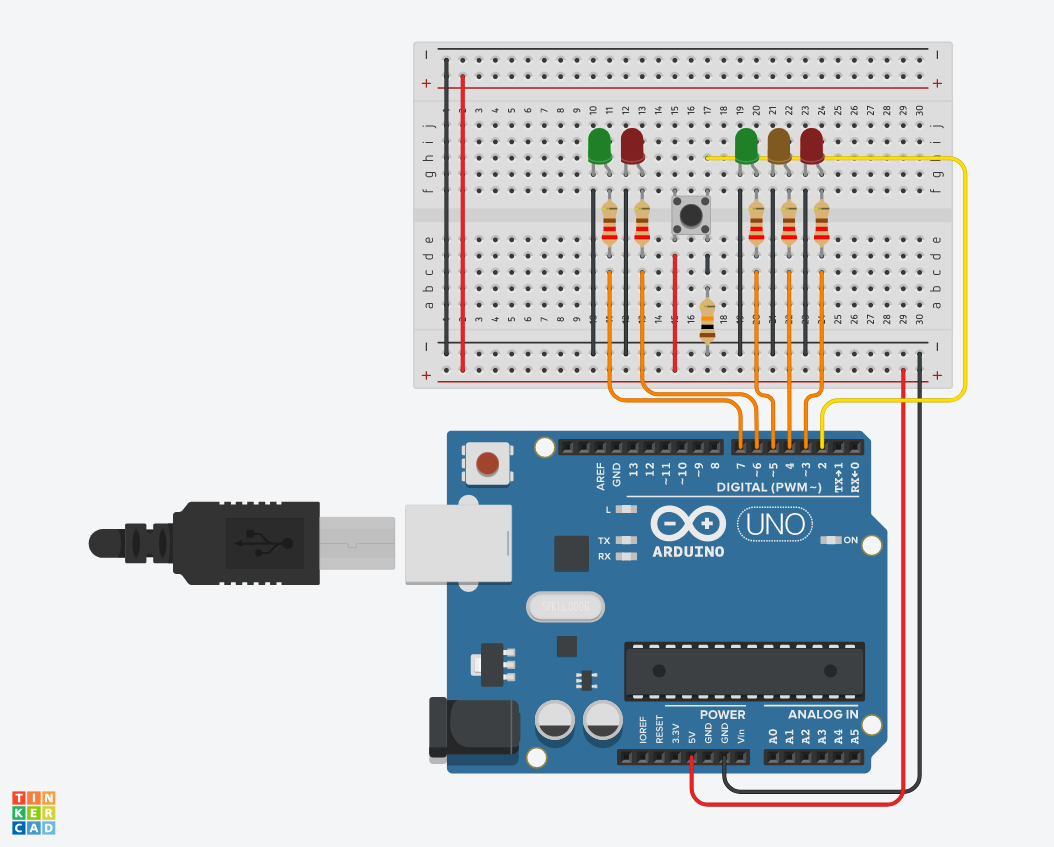
\includegraphics[width=\linewidth]{traffic.png}
\pagebreak

\section{Κώδικας}

\lstinputlisting[language=C]{traffic.ino}

\section{Πίνακας καταστάσεων}

\begin{itemize}
	\item $P_1$: Κόκκινο πεζών
	\item $P_2$: Πράσινο πεζών
	\item $T_1$: Κόκκινο οχημάτων
	\item $T_2$: Πορτοκαλί οχημάτων
	\item $T_3$: Πράσινο οχημάτων
\end{itemize}

\begin{center}
\begin{tabular}{|l|l|l|l|l|}
	\hline
	$P_1$ & $P_2$ & $T_1$ & $T_2$ & $T_3$ \\
	\hline
	1 & 0 & 0 & 0 & 1 \\
	\hline
	1 & 0 & 0 & 1 & 0 \\
	\hline
	0 & 1 & 1 & 0 & 0 \\
	\hline
	1 & 0 & 1 & 0 & 0 \\
	\hline
\end{tabular}
\end{center}

\end{document}
